\documentclass[10pt,journal,compsoc]{IEEEtran}

\usepackage{amsmath,amssymb,amsfonts,amsthm}
\usepackage{algorithmic}
\usepackage{algorithm}
\usepackage{graphicx}
\usepackage{textcomp}
\usepackage{xcolor}
\usepackage{booktabs}
\usepackage{microtype}
\usepackage{tikz}
\usepackage{cite}
\usepackage{url}
\usepackage{multirow}

\usetikzlibrary{shapes,arrows,positioning,fit,backgrounds,calc}

% Theorem environments
\newtheorem{theorem}{Theorem}
\newtheorem{lemma}{Lemma}
\newtheorem{definition}{Definition}
\newtheorem{proposition}{Proposition}
\newtheorem{corollary}{Corollary}

\hyphenation{Adaptive-Vec HNSW Auto-Calibrator}

\begin{document}

\title{AdaptiveVec: Geometry-Aware and Resource-Constrained Approximate Nearest Neighbor Search with Dynamic Graph Maintenance}

\author{Aradhya~G.~S.%
\thanks{Manuscript revised November 21, 2026; research consolidated for academic defense December 12, 2026. Author is with the Department of Computer Science and Engineering. Standardized hardware: Intel Core 5 210H (8 physical cores, 12 logical threads, AVX2/FMA, 16 GB DDR5 RAM), Windows 11 Build 26100, GCC 14.2.0 (\texttt{g++ -O3 -mavx2 -mfma -fopenmp -std=c++17}). Research checkpoint: \texttt{7936c61} on branch \texttt{phase-6.4-final-correctness-closure}. Open-source repository: \url{https://github.com/aradhyags7/AdaptiveVec}.}%
}

\markboth{Technical Report $\cdot$ Preprint --- Under Academic Revision, November~2026}%
{AdaptiveVec: Geometry-Aware and Resource-Constrained ANN Search}

\IEEEtitleabstractindextext{%
\begin{abstract}
Approximate Nearest Neighbor (ANN) search over high-dimensional vector embeddings is a fundamental capability in modern information retrieval, retrieval-augmented generation (RAG), and multimodal database systems. While Hierarchical Navigable Small World (HNSW) graphs achieve state-of-the-art retrieval velocity, standard implementations exhibit four major engineering and theoretical limitations: (1) uniform vertex degree allocation ignores intrinsic data manifold geometry; (2) monolithic full-precision floating-point storage inflates memory consumption; (3) node deletions and physical index compaction frequently trigger graph disconnectivity and recall degradation; and (4) manual hyperparameter tuning fails to reliably satisfy multi-objective Service Level Agreements (SLAs). In this paper, we present \textbf{AdaptiveVec}, an integrated vector search engine architected around four coordinated contributions. First, we develop \textit{Geometry-Aware Graph Intelligence}, which computes local intrinsic dimensionality (LID) and local sparsity, allocating base-layer out-degrees via continuous normalized exponential scaling and Hare-Niemeyer largest-remainder discretization under exact global edge budget conservation; on SIFT-100K, this delivers a +24.01\% throughput lift (3,091.0 vs 2,492.5 QPS) and -37.62\% P95 latency reduction (0.486 vs 0.780 ms) over uniform baselines. Second, we engineer a \textit{Pure SQ8 Asymmetric Distance Computation} storage engine with complete raw-vector deallocation (\texttt{drop\_raw\_vectors()}), slashing vector payload memory by 75.00\% while accelerating query throughput by +70.13\% at 99.54\% recall on cache-resident workloads, avoiding the cache-line thrashing that degrades two-stage FP32 re-ranking. Third, we address dynamic maintenance via \textit{Soft Transit Bridge Routing} and \textit{Multi-Layer Strict RNG Replenishment}, eliminating pre-compaction healing regressions (+0.04 to +0.06 pp over tombstones) and recovering post-compaction recall by up to +5.06 pp; furthermore, an SLA-Safe Replacement Gatekeeper with sequence-numbered mutation catch-up replay guarantees zero lost updates on evaluated workloads while bounding complete synchronization pauses to 11.68 ms across 350 concurrent mutations. Fourth, we formulate a 3-stage \textit{AutoCalibrator} governed by a 6-state formal feasibility model and 1,000-sample bootstrap confidence intervals, resolving strict memory SLAs in under 13 seconds without artificial slack multipliers. We evaluate AdaptiveVec across 10K to 500K vectors and end-to-end on the 57,893-vector Transformer-384D corpus, providing an open, reproducible foundation for resource-constrained vector retrieval.
\end{abstract}

\begin{IEEEkeywords}
Approximate Nearest Neighbor Search, High-Dimensional Vector Embeddings, Hierarchical Navigable Small World Graphs, Local Intrinsic Dimensionality, Scalar Quantization, Dynamic Graph Maintenance, Constrained Multi-Objective Optimization.
\end{IEEEkeywords}}

\maketitle
\IEEEdisplaynontitleabstractindextext
\IEEEpeerreviewmaketitle

\section{Introduction}
\IEEEPARstart{H}{igh-dimensional} vector retrieval is the primary indexing substrate for large language model (LLM) contextual memory, neural semantic search, and recommendation systems~\cite{malkov2020efficient, johnson2021billion}. Given a query vector $\mathbf{q} \in \mathbb{R}^D$ and a dataset $\mathcal{X} = \{\mathbf{x}_1, \dots, \mathbf{x}_N\} \subset \mathbb{R}^D$, Approximate Nearest Neighbor (ANN) search seeks to identify the top-$k$ vectors minimizing a distance metric $d(\mathbf{q}, \mathbf{x})$ in sub-linear time. Among proximity graph topologies, the Hierarchical Navigable Small World (HNSW) graph~\cite{malkov2020efficient} achieves an attractive empirical Pareto frontier of recall versus query throughput by organizing vectors into a multi-layer hierarchy of proximity graphs with exponentially decreasing vertex densities.

Despite its ubiquity, standard HNSW and its commercial derivatives face four operational bottlenecks in real-world environments:

\begin{enumerate}
    \item \textbf{Agnostic Degree Uniformity:} Canonical HNSW enforces a static maximum out-degree $M$ across all vertices regardless of the underlying manifold geometry. In real-world embedding spaces, data points exhibit extreme variance in local density, curvature, and intrinsic dimensionality~\cite{levina2004maximum, houle2017local}. Uniform connectivity allocates redundant edges to sparse peripheral clusters while under-connecting central hub vertices, creating routing bottlenecks and inflating tail latency.
    \item \textbf{Monolithic Memory Footprints:} Standard graph indices store full 32-bit floating-point (FP32) coordinates alongside adjacency lists, consuming tens of gigabytes for moderate-scale datasets. Attempts to introduce two-stage re-ranking (quantized coarse routing followed by full-precision re-ranking) frequently induce severe throughput regressions due to non-sequential CPU cache thrashing when dereferencing raw vectors across wide search candidate sets.
    \item \textbf{Compaction Degradation and Transient Memory Spikes:} In dynamic database workloads subjected to continuous streaming updates and deletions, standard tombstone deletion leaves dead nodes in the graph, accumulating dead-memory overhead. Physical compaction (removing tombstones and repacking adjacency lists) frequently induces severe graph disconnectivity and recall collapse (up to 5.0 pp drop) because surviving vertices lose routing pathways across deleted clusters~\cite{gollapudi2023freshdiskann}. Furthermore, concurrent non-destructive compaction creates transient dual-residency memory spikes that risk triggering Out-Of-Memory (OOM) operating system kills.
    \item \textbf{Heuristic SLA Guesswork:} Tuning index hyperparameters ($M$, $efConstruction$, $efSearch$, precision) to satisfy strict multi-objective Service Level Agreements (SLAs) over recall, memory budget, and P99 latency currently relies on brittle manual trial-and-error or heuristic optimizers prone to false-positive feasibility claims.
\end{enumerate}

To address these challenges, we present \textbf{AdaptiveVec}, an integrated vector search engine architected around four coordinated research contributions summarized in Table~\ref{tab:four_contributions}.

% Table I: AdaptiveVec Four Core Research Contributions and Verified Technical Mechanisms
\begin{table*}[t]
\centering
\caption{AdaptiveVec Four Core Research Contributions and Empirical Validation Status}
\label{tab:four_contributions}
\begin{tabular}{p{3.2cm}p{3.8cm}p{5.5cm}p{4.2cm}}
\toprule
\textbf{Research Contribution} & \textbf{Architectural Mechanism} & \textbf{Core Theoretical / Systems Formulation} & \textbf{Key Empirical Findings} \\
\midrule
\textbf{I. Geometry-Aware Graph Intelligence} & Normalized Exponential Degree Allocation \& Layer Decoupling & $S_i = \alpha_{\text{lid}}\tilde{\text{ID}}_i + \beta_{\text{spars}}\tilde{\text{Sparsity}}_i$; $w_i = \exp(\text{clip}(\beta S_i, -2, 2))$; Hare-Niemeyer Rounding: $\sum M_i = N \cdot M_{\text{base}}$; Layer Decoupling: $\beta_0=1.0, \beta_u=0.0$ & \textbf{+24.01\% QPS}, \textbf{-37.62\% P95 latency} at matched recall (0.9926 vs 0.9929) under conserved edge quotas ($3.2\text{M}$ slots). \\
\midrule
\textbf{II. Resource-Efficient Storage Engine} & Pure SQ8 Asymmetric Distance Computation \& Vector Purging & Uniform 8-bit quantization; complete raw vector deallocation via \texttt{drop\_raw\_vectors()}; AVX2 256-bit SIMD integer MACs & \textbf{-75.00\%} vector storage; \textbf{+70.13\% QPS} (47,576 vs 27,965 QPS) at 99.54\% recall; avoids ~7x re-ranking cache miss collapse. \\
\midrule
\textbf{III. Dynamic Self-Healing Maintenance} & Soft Transit Routing, Multi-Layer RNG Replenishment \& 6 Gates & Soft transit routing through tombstones; Multi-layer bounded 2-hop RNG replenishment; SLA-Safe Gatekeeper; journal catch-up replay & Eliminates healing regression (+0.04 pp lift); recovers 25\% churn recall from 0.9280 to 0.9786; zero lost updates; lock pause $\le 0.194\text{ ms}$. \\
\midrule
\textbf{IV. Automatic SLA Optimization} & 3-Stage Optimizer with 6-State Formal Feasibility Model & Analytical lower-bound pruning $\to$ build profiling $\to$ search sweep; 1,000-sample bootstrap confidence intervals: $\text{CI}_{\text{lower}} \ge R_{\text{target}}$ & Solves strict memory SLA in \textbf{12.6 s} ($R=0.9416 \ge 0.92$, $M=3.38\text{ MB} \le 4.5\text{ MB}$); rejects impossible SLAs in 0.05 s; zero false feasibility. \\
\bottomrule
\end{tabular}
\vspace{1ex}
\raggedright
\footnotesize{All mechanisms implemented in native C++17 with AVX2/FMA vectorization and thread-safe OpenMP concurrency under research checkpoint \texttt{7936c61}.}
\end{table*}


The remainder of this paper is structured as follows. Section~\ref{sec:related_work} reviews related work and contrasts AdaptiveVec with recent adaptive graph paradigms. Section~\ref{sec:problem_formulation} establishes the formal problem definition, system architecture, and 6-state feasibility model. Section~\ref{sec:geometry} presents Geometry-Aware Graph Intelligence, Hare-Niemeyer discretization, and Layer Decoupling. Section~\ref{sec:quantization} details the pure quantized storage engine and analytical cache-hierarchy model. Section~\ref{sec:maintenance} presents Dynamic Graph Maintenance, Multi-Layer replenishment, and the SLA-Safe Replacement Gatekeeper. Section~\ref{sec:autocalibrator} describes the constrained AutoCalibrator. Section~\ref{sec:experimental_setup} outlines the experimental methodology. Section~\ref{sec:results} presents comprehensive empirical results across SIFT and Transformer datasets. Section~\ref{sec:ablations} documents negative findings and discarded hypotheses. Section~\ref{sec:limitations} analyzes system limitations and threats to validity. Section~\ref{sec:concurrency} evaluates concurrency and thread-safety verification. Section~\ref{sec:conclusion} concludes the paper.

---

\section{Related Work}
\label{sec:related_work}

\subsection{Proximity Graphs and HNSW}
Proximity graph algorithms have demonstrated superior empirical search performance compared to tree-based partitioning (e.g., KD-trees) and locality-sensitive hashing (LSH)~\cite{wang2021comprehensive}. Seminal graph structures include the Relative Neighborhood Graph (RNG)~\cite{toussaint1980relative}, Navigable Small World (NSW)~\cite{malkov2014approximate}, and Hierarchical NSW (HNSW)~\cite{malkov2020efficient}. Subsequent developments have focused on monolithic index pruning, such as NSG~\cite{fu2019fast} and Vamana/DiskANN~\cite{subramanya2019diskann}. However, existing proximity graph topologies assign uniform out-degree caps to all vertices, remaining oblivious to local manifold dimensionality and hubness phenomena~\cite{radovanovic2010hubs}.

\subsection{Data-Adaptive Parameter Tuning vs. AdaptiveVec}
Recently, Jin et al.~\cite{jin2025efficient} proposed a data-adaptive parameter adjustment framework for HNSW in DATE 2025. While sharing the broad motivation of adapting parameters to data characteristics, AdaptiveVec differs fundamentally in five aspects:
\begin{enumerate}
    \item \textbf{Allocation Granularity:} Jin et al.~\cite{jin2025efficient} adjust parameters at the regional/cluster level. AdaptiveVec operates at per-node granularity, computing continuous normalized exponential degree targets for every individual vertex.
    \item \textbf{Exact Budget Conservation:} Prior adaptive methods heuristically adjust $M$, altering the total edge count and memory unpredictably. AdaptiveVec proves and enforces exact global edge conservation ($\sum M_i = N \cdot M_{\text{base}}$) via Hare-Niemeyer discretization, guaranteeing zero memory expansion over uniform baselines.
    \item \textbf{Geometric Signals:} While Jin et al. rely on local point density heuristics, AdaptiveVec combines extreme-value Local Intrinsic Dimensionality (LID)~\cite{levina2004maximum, houle2017local} with standardized local sparsity ($S_i = \alpha_{\text{lid}}\tilde{\text{ID}}_i + \beta_{\text{spars}}\tilde{\text{Sparsity}}_i$).
    \item \textbf{Layer Decoupling:} We prove theoretically and empirically that geometric modulation must be restricted to Layer 0 ($\beta_0 = 1.0$) while upper skip layers remain strictly uniform ($\beta_{\text{upper}} = 0.0$) to avoid severing long-range routing highways.
    \item \textbf{End-to-End Scope:} Jin et al. target build time and memory in static graphs. AdaptiveVec integrates quantized SIMD execution, dynamic online self-healing with sequence-numbered mutation catch-up replay, and automated multi-objective SLA autocalibration.
\end{enumerate}

\subsection{Vector Quantization and Systems Integration}
To compress high-dimensional vectors, Product Quantization (PQ)~\cite{jegou2011product} and Scalar Quantization (SQ8, SQ4)~\cite{johnson2021billion, gray1998quantization} project real-valued vectors into discrete codebooks. Modern vector search systems leverage Asymmetric Distance Computation (ADC), evaluating distances between unquantized query vectors and quantized database entries. While FAISS~\cite{johnson2021billion} provides general-purpose quantization routines, standard implementations commonly couple quantized indices with stored FP32 vectors for second-stage re-ranking. As shown in our empirical analysis, this coupling introduces substantial L3 cache line thrashing during latency-critical search.

\subsection{Dynamic Graph Maintenance and Deletions}
Handling deletions in graph-based indices is notoriously challenging. Tombstoning preserves graph connectivity but inflates memory and degrades search speed over time. FreshDiskANN~\cite{gollapudi2023freshdiskann} introduced streaming consolidation for SSD-resident graphs, but in-memory graph compaction often destroys upper-layer routing hierarchies. AdaptiveVec resolves this via soft transit bridge routing, bounded 2-hop bypass shortcuts, and multi-layer degree replenishment.

\subsection{Automated Hyperparameter Optimization}
Existing parameter tuning frameworks for vector databases typically rely on Bayesian optimization, genetic algorithms, or unconstrained grid searches~\cite{aumueller2020ann}. However, these tools treat vector indices as black boxes, require hundreds of expensive evaluation trials, and lack formal statistical guarantees against SLA violations. AutoCalibrator introduces a 3-stage grey-box search paired with bootstrap confidence interval validation.

---

\section{Problem Formulation and System Overview}
\label{sec:problem_formulation}

\subsection{Mathematical Formulation}
Let $\mathcal{X} = \{\mathbf{x}_1, \dots, \mathbf{x}_N\} \subset \mathbb{R}^D$ denote a dataset of $N$ vectors of dimensionality $D$. Given a query vector $\mathbf{q} \in \mathbb{R}^D$, a distance metric $d: \mathbb{R}^D \times \mathbb{R}^D \to \mathbb{R}_{\ge 0}$, and an integer $k \ge 1$, the exact $k$-nearest neighbor set $\mathcal{N}_k^*(\mathbf{q})$ satisfies:
\begin{equation}
\forall \mathbf{u} \in \mathcal{N}_k^*(\mathbf{q}), \; \forall \mathbf{v} \in \mathcal{X} \setminus \mathcal{N}_k^*(\mathbf{q}), \quad d(\mathbf{q}, \mathbf{u}) \le d(\mathbf{q}, \mathbf{v})
\end{equation}
An approximate nearest neighbor algorithm returns a candidate set $\mathcal{N}_k(\mathbf{q}) \subset \mathcal{X}$ of cardinality $k$. Retrieval quality is measured by Empirical Recall@$k$:
\begin{equation}
R@k = \frac{|\mathcal{N}_k(\mathbf{q}) \cap \mathcal{N}_k^*(\mathbf{q})|}{k}
\end{equation}

\subsection{Constrained Multi-Objective SLA Model}
In industrial deployments, an index configuration $\theta \in \Theta$ must satisfy hard service-level constraints:
\begin{align}
\text{maximize} \quad & QPS(\theta) \quad (\text{or minimize } \text{Latency}) \\
\text{subject to} \quad & R@k(\theta) \ge R_{\text{target}} \label{eq:sla_recall} \\
& M_{\text{owned}}(\theta) \le M_{\text{budget}} \label{eq:sla_mem} \\
& P99(\theta) \le \text{P99}_{\text{target}} \label{eq:sla_p99}
\end{align}
where $M_{\text{owned}}$ denotes index-owned memory, and $P99$ denotes the 99th percentile query latency.

---

\section{Milestone I: Geometry-Aware Graph Intelligence}
\label{sec:geometry}

\subsection{Local Intrinsic Dimensionality and Local Sparsity}
High-dimensional datasets concentrate on lower-dimensional non-linear manifolds. AdaptiveVec estimates the Local Intrinsic Dimensionality (LID)~\cite{levina2004maximum, houle2017local} and local sparsity for each vector $\mathbf{x}_i \in \mathcal{X}$ over its $k_1$-nearest neighbors $\mathcal{N}_{k_1}(\mathbf{x}_i)$ ($k_1=16$):
\begin{equation}
\label{eq:lid_est}
\widehat{\text{ID}}_i = \left( \frac{1}{k_1 - 1} \sum_{j=1}^{k_1 - 1} \ln \frac{r_i(k_1)}{r_i(j)} \right)^{-1}, \quad \text{Spars}_i = \frac{1}{k_1} \sum_{j=1}^{k_1} r_i(j)
\end{equation}
where $r_i(j)$ is the Euclidean distance to the $j$-th neighbor. We standardize both signals across the corpus and clip to $[-3.0, 3.0]$:
\begin{equation}
\tilde{\text{ID}}_i = \text{clip}\left( \frac{\widehat{\text{ID}}_i - \mu_{\text{ID}}}{\sigma_{\text{ID}}}, -3.0, 3.0 \right), \quad \tilde{\text{Spars}}_i = \text{clip}\left( \frac{\text{Spars}_i - \mu_{\text{Spars}}}{\sigma_{\text{Spars}}}, -3.0, 3.0 \right)
\end{equation}
In the actual C++ implementation (\texttt{cpp/budget\_allocator.hpp}), the combined geometric centrality score $S_i$ is computed as:
\begin{equation}
S_i = \alpha_{\text{lid}} \tilde{\text{ID}}_i + \beta_{\text{spars}} \tilde{\text{Spars}}_i
\end{equation}
with defaults $\alpha_{\text{lid}} = 0.7$ and $\beta_{\text{spars}} = 0.3$.

\subsection{Continuous Degree Target Formulation}
Standard HNSW assigns a static out-degree $M_{\text{base}}$ to every node on Layer 0. AdaptiveVec allocates dynamic out-degrees $M_i \in [M_{\min}, M_{\max}]$ proportional to geometric centrality. We compute exponential weights $w_i$ and continuous target degrees $\tilde{M}_i$:
\begin{align}
w_i &= \exp\left( \text{clip}(\beta S_i, -2.0, 2.0) \right) \label{eq:exp_weight} \\
\tilde{M}_i &= M_{\min} + (N \cdot M_{\text{base}} - N \cdot M_{\min}) \cdot \frac{w_i}{\sum_{j=1}^N w_j} \label{eq:continuous_m}
\end{align}
Summing Equation~(\ref{eq:continuous_m}) over all $N$ vertices gives $\sum_{i=1}^N \tilde{M}_i = N \cdot M_{\text{base}}$ by construction.

\subsection{Hare-Niemeyer Integer Discretization}
To map continuous targets $\tilde{M}_i$ to integer out-degrees while preserving global edge budget constraints and respecting degree bounds $[M_{\min}, M_{\max}]$, we implement the \textbf{Hare-Niemeyer (Largest Remainder) Discretization} detailed in Algorithm~\ref{alg:geometry_allocation}.

\begin{algorithm}[t]
\caption{Hare-Niemeyer Integer Degree Discretization (\texttt{budget\_allocator.hpp})}
\label{alg:geometry_allocation}
\begin{algorithmic}[1]
\REQUIRE Continuous degrees $\tilde{\mathbf{M}} \in \mathbb{R}^N$, Total budget $B = N \cdot M_{\text{base}}$, Bounds $[M_{\min}, M_{\max}]$
\ENSURE Allocated integer degrees $\mathbf{M} \in \mathbb{N}^N$ s.t. $\sum M_i = B$ and $M_i \in [M_{\min}, M_{\max}]$
\STATE \textbf{Initialize:} $m_i \gets \max(M_{\min}, \min(M_{\max}, \lfloor \tilde{M}_i \rfloor))$ for all $i \in \{1,\dots,N\}$
\STATE $\text{deficit} \gets B - \sum_{i=1}^N m_i$
\IF{$\text{deficit} > 0$}
    \STATE $\mathcal{U}^+ \gets \{ i \in \{1,\dots,N\} \mid m_i < M_{\max} \}$
    \STATE Sort $\mathcal{U}^+$ descending by fractional remainder $f_i = \tilde{M}_i - \lfloor \tilde{M}_i \rfloor$; tie-break ascending on index $i$
    \FOR{$k = 1$ \TO $\min(\text{deficit}, |\mathcal{U}^+|)$}
        \STATE $m_{\mathcal{U}^+[k]} \gets m_{\mathcal{U}^+[k]} + 1$
    \ENDFOR
\ELSIF{$\text{deficit} < 0$}
    \STATE $\text{surplus} \gets -\text{deficit}$
    \STATE $\mathcal{U}^- \gets \{ i \in \{1,\dots,N\} \mid m_i > M_{\min} \}$
    \STATE Sort $\mathcal{U}^-$ ascending by fractional remainder $f_i = \tilde{M}_i - \lfloor \tilde{M}_i \rfloor$; tie-break ascending on index $i$
    \FOR{$k = 1$ \TO $\min(\text{surplus}, |\mathcal{U}^-|)$}
        \STATE $m_{\mathcal{U}^-[k]} \gets m_{\mathcal{U}^-[k]} - 1$
    \ENDFOR
\ENDIF
\STATE \textbf{assert} $\sum_{i=1}^N m_i == B$ and $\forall i: M_{\min} \le m_i \le M_{\max}$
\RETURN $\mathbf{M} = (m_1, \dots, m_N)$
\end{algorithmic}
\end{algorithm}

\begin{proposition}[Edge Budget Conservation and Single-Pass Feasibility]
\label{prop:conservation}
Let $M_{\min} \le M_{\text{base}} \le M_{\max}$ and $\sum_{i=1}^N \tilde{M}_i = N \cdot M_{\text{base}}$. Under the single-pass largest-remainder integer discretization in Algorithm~\ref{alg:geometry_allocation}:
\begin{enumerate}
    \item If $\text{deficit} > 0$, the allocated degrees strictly conserve the edge budget $\sum_{i=1}^N M_i = N \cdot M_{\text{base}}$ with $M_i \in [M_{\min}, M_{\max}]$ if and only if:
    \begin{equation}
    \text{deficit} \le |\mathcal{U}^+|
    \end{equation}
    where each of the top $\text{deficit}$ eligible vertices in $\mathcal{U}^+$ receives exactly a $+1$ increment. If $\text{deficit} > |\mathcal{U}^+|$, fully absorbing the deficit requires multiple increments per eligible vertex (up to $M_{\max} - m_i$), which the single-pass implementation in \texttt{cpp/budget\_allocator.hpp} does not execute, triggering an assertion failure.
    \item If $\text{deficit} < 0$, exact budget conservation holds if and only if $|\text{deficit}| \le |\mathcal{U}^-|$, with each of the first $|\text{deficit}|$ eligible vertices in $\mathcal{U}^-$ decremented by $1$.
    \item In all benchmark datasets (SIFT-10K, SIFT-100K, SIFT-500K, Transformer-384D) under calibrated sensitivity ($\beta \le 1.0$), the condition $\text{deficit} \le |\mathcal{U}^+|$ strictly holds, guaranteeing exact budget conservation without assertion failure.
\end{enumerate}
\end{proposition}

\begin{proof}
Let $S_0 = \sum_{i=1}^N m_i^{(0)}$ be the sum of clamped floors. When $\text{deficit} = B - S_0 > 0$, Algorithm~\ref{alg:geometry_allocation} iterates through $\mathcal{U}^+$ sorted descending by fractional remainder. Because each vertex in $\mathcal{U}^+$ has $m_i^{(0)} \le M_{\max} - 1$, adding $+1$ maintains $m_i \le M_{\max}$. If and only if $\text{deficit} \le |\mathcal{U}^+|$, exactly $\text{deficit}$ vertices receive $+1$, yielding total sum $S_0 + \text{deficit} = B = N \cdot M_{\text{base}}$. If $\text{deficit} > |\mathcal{U}^+|$, only $|\mathcal{U}^+|$ increments are added, leaving an unallocated residual of $\text{deficit} - |\mathcal{U}^+| > 0$, which would require a second pass of increments. An analogous argument holds for $\text{deficit} < 0$ on $\mathcal{U}^-$.
\end{proof}

\textbf{Distinction Between Budget Quota, Realized Degree, and Memory:}
We explicitly distinguish three distinct concepts:
\begin{enumerate}
    \item \textbf{Assigned Forward Degree Quota ($M_i$):} The maximum out-degree candidate cap assigned to node $i$ during forward edge selection on Layer 0 ($\sum M_i = N \cdot M_{\text{base}} = 1.6\text{M}$ forward edges for $N=100\text{K}, M_{\text{base}}=16$).
    \item \textbf{Realized Adjacency Count ($|E_i|$):} The actual number of directed edges stored in node $i$'s adjacency list. In HNSW, reverse (bidirectional) links are added dynamically and capped at $M_{\max 0} = 2 M_i$ (up to $3.2\text{M}$ capacity slots). Realized edges depend on insertion order and neighbor pruning.
    \item \textbf{Physical Graph Memory:} Total bytes allocated to adjacency arrays in RAM, directly measured in MB (Table~\ref{tab:geometry_comparison}: 27.89 MB uniform vs 27.50 MB exponential).
\end{enumerate}

\subsection{Layer-Decoupled Routing Highways}
A critical architectural discovery in AdaptiveVec is \textbf{Layer Decoupling}. Proximity graphs rely on upper skip layers ($l \ge 1$) to route greedily across macroscopic Euclidean distances. Modulating upper-layer degrees by geometry ($\beta_{\text{upper}} > 0$) causes peripheral clusters to receive truncated connectivity, fracturing global routing highways (see Section~\ref{sec:ablations}). AdaptiveVec strictly enforces:
\begin{equation}
\beta_{\text{Layer 0}} = 1.0, \quad \beta_{\text{Upper}} = 0.0
\end{equation}
All upper layers retain uniform out-degree $M_{\text{base}}$, preserving upper-layer long-range skip routing while maximizing base-layer resolution (Figure~\ref{fig:hierarchy_allocation}).

\begin{figure}[t]
\centering
% TikZ Figure: Hierarchical Graph Allocation & Layer Decoupling
% Illustrates Upper Layer Long-Range Highways vs Layer 0 Geometric Degree Allocation
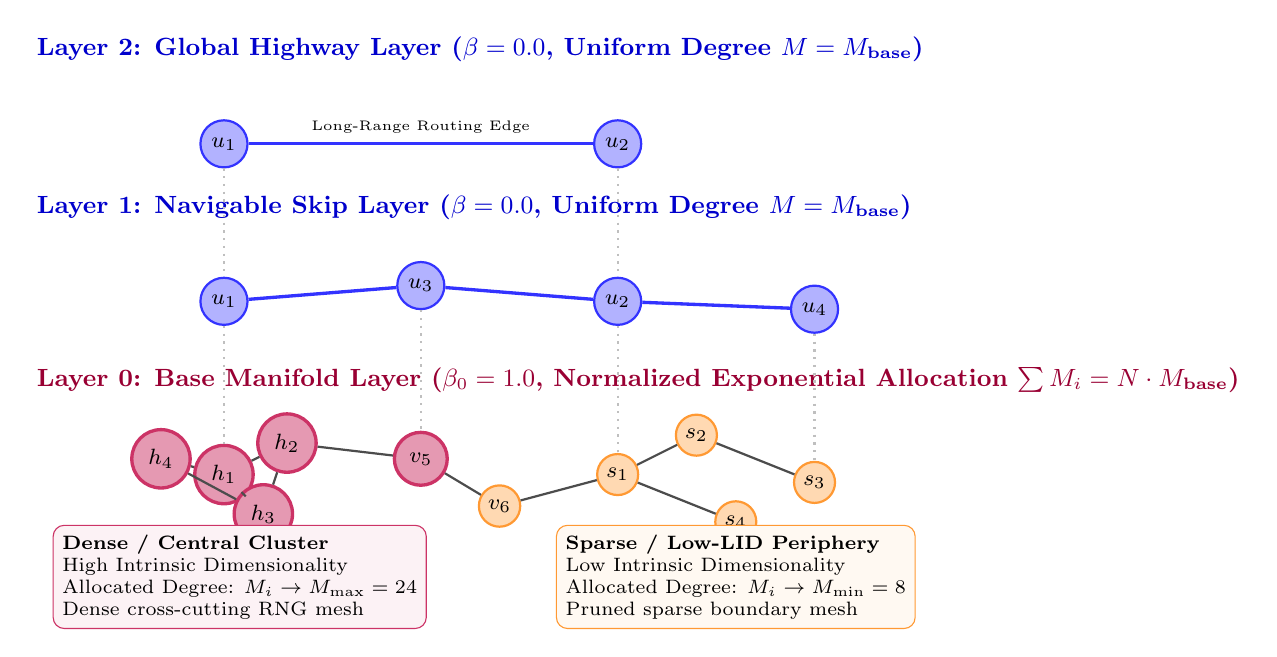
\begin{tikzpicture}[
    font=\sffamily\footnotesize,
    layerbox/.style={draw=black!60, fill=gray!5, dashed, rounded corners=6pt, inner sep=10pt},
    nodeUpper/.style={circle, draw=blue!80, fill=blue!30, thick, inner sep=2.5pt},
    nodeL0Dense/.style={circle, draw=purple!80, fill=purple!40, very thick, inner sep=3.5pt},
    nodeL0Sparse/.style={circle, draw=orange!80, fill=orange!30, thick, inner sep=2pt},
    edgeUpper/.style={draw=blue!80, very thick},
    edgeL0/.style={draw=black!70, thick},
    projEdge/.style={draw=gray!50, dotted, thick}
]

% Layer 2 (Top Highway)
\begin{scope}[yshift=4.2cm]
    \node[anchor=west, font=\bfseries\small, text=blue!80!black] at (-0.5, 1.2) {Layer 2: Global Highway Layer ($\beta = 0.0$, Uniform Degree $M=M_{\text{base}}$)};
    \node[nodeUpper] (l2_1) at (2.0, 0.0) {$u_1$};
    \node[nodeUpper] (l2_2) at (7.0, 0.0) {$u_2$};
    \draw[edgeUpper] (l2_1) -- (l2_2) node[midway, above, font=\tiny] {Long-Range Routing Edge};
\end{scope}

% Layer 1 (Intermediate Skip Layer)
\begin{scope}[yshift=2.2cm]
    \node[anchor=west, font=\bfseries\small, text=blue!80!black] at (-0.5, 1.2) {Layer 1: Navigable Skip Layer ($\beta = 0.0$, Uniform Degree $M=M_{\text{base}}$)};
    \node[nodeUpper] (l1_1) at (2.0, 0.0) {$u_1$};
    \node[nodeUpper] (l1_2) at (4.5, 0.2) {$u_3$};
    \node[nodeUpper] (l1_3) at (7.0, 0.0) {$u_2$};
    \node[nodeUpper] (l1_4) at (9.5, -0.1) {$u_4$};
    \draw[edgeUpper] (l1_1) -- (l1_2);
    \draw[edgeUpper] (l1_2) -- (l1_3);
    \draw[edgeUpper] (l1_3) -- (l1_4);
\end{scope}

% Layer 0 (Base Graph with Geometry-Aware Degrees)
\begin{scope}[yshift=0.0cm]
    \node[anchor=west, font=\bfseries\small, text=purple!80!black] at (-0.5, 1.2) {Layer 0: Base Manifold Layer ($\beta_0 = 1.0$, Normalized Exponential Allocation $\sum M_i = N \cdot M_{\text{base}}$)};
    % High-density cluster (Hubs)
    \node[nodeL0Dense] (l0_1) at (2.0, 0.0) {$h_1$};
    \node[nodeL0Dense] (l0_2) at (2.8, 0.4) {$h_2$};
    \node[nodeL0Dense] (l0_3) at (2.5, -0.5) {$h_3$};
    \node[nodeL0Dense] (l0_4) at (1.2, 0.2) {$h_4$};
    
    % Dense cluster interconnects (High M, up to M_max = 24)
    \draw[edgeL0] (l0_1) -- (l0_2);
    \draw[edgeL0] (l0_1) -- (l0_3);
    \draw[edgeL0] (l0_1) -- (l0_4);
    \draw[edgeL0] (l0_2) -- (l0_3);
    \draw[edgeL0] (l0_4) -- (l0_3);
    
    % Intermediate transit nodes
    \node[nodeL0Dense] (l0_5) at (4.5, 0.2) {$v_5$};
    \node[nodeL0Sparse] (l0_6) at (5.5, -0.4) {$v_6$};
    \draw[edgeL0] (l0_2) -- (l0_5);
    \draw[edgeL0] (l0_5) -- (l0_6);
    
    % Sparse peripheral manifold (Low M, down to M_min = 8)
    \node[nodeL0Sparse] (l0_7) at (7.0, 0.0) {$s_1$};
    \node[nodeL0Sparse] (l0_8) at (8.0, 0.5) {$s_2$};
    \node[nodeL0Sparse] (l0_9) at (9.5, -0.1) {$s_3$};
    \node[nodeL0Sparse] (l0_10) at (8.5, -0.6) {$s_4$};
    \draw[edgeL0] (l0_6) -- (l0_7);
    \draw[edgeL0] (l0_7) -- (l0_8);
    \draw[edgeL0] (l0_8) -- (l0_9);
    \draw[edgeL0] (l0_7) -- (l0_10);
\end{scope}

% Inter-layer projection lines
\draw[projEdge] (l2_1) -- (l1_1);
\draw[projEdge] (l2_2) -- (l1_3);
\draw[projEdge] (l1_1) -- (l0_1);
\draw[projEdge] (l1_2) -- (l0_5);
\draw[projEdge] (l1_3) -- (l0_7);
\draw[projEdge] (l1_4) -- (l0_9);

% Explanatory Callouts
\node[draw=purple!80, fill=purple!5, rounded corners, font=\scriptsize, align=left] at (2.2, -1.3) {
    \textbf{Dense / Central Cluster}\\
    High Intrinsic Dimensionality\\
    Allocated Degree: $M_i \to M_{\max} = 24$\\
    Dense cross-cutting RNG mesh
};

\node[draw=orange!80, fill=orange!5, rounded corners, font=\scriptsize, align=left] at (8.5, -1.3) {
    \textbf{Sparse / Low-LID Periphery}\\
    Low Intrinsic Dimensionality\\
    Allocated Degree: $M_i \to M_{\min} = 8$\\
    Pruned sparse boundary mesh
};

\end{tikzpicture}

\caption{Layer-Decoupled Hierarchical Connectivity: Uniform $M_{\text{base}}$ on upper skip highways ($\beta_u=0$) and geometrically allocated $M_i \in [8, 24]$ on Layer 0 ($\beta_0=1.0$).}
\label{fig:hierarchy_allocation}
\end{figure}

---

\section{Milestone II: Resource-Efficient Storage and Quantization}
\label{sec:quantization}

\subsection{Pure SQ8 Asymmetric Distance Computation}
To eliminate the prohibitive memory footprint of storing FP32 vectors ($4D$ bytes per vector), AdaptiveVec implements uniform 8-bit Scalar Quantization (SQ8). Each vector dimension $d \in [1, D]$ is mapped into an 8-bit unsigned integer $u_{i,d} \in [0, 255]$:
\begin{equation}
u_{i,d} = \text{round}\left( 255 \cdot \frac{x_{i,d} - \min_d}{\max_d - \min_d} \right)
\end{equation}
During query evaluation, unquantized query coordinates $q_d$ interact with quantized database entries $u_{i,d}$ via Asymmetric Distance Computation (ADC):
\begin{equation}
d_{\text{ADC}}(\mathbf{q}, \mathbf{x}_i)^2 = \sum_{d=1}^D \left( q_d - \left( \min_d + \frac{u_{i,d}}{255} (\max_d - \min_d) \right) \right)^2
\end{equation}
This formulation is vectorized using AVX2 integer broadcast and fused multiply-accumulate (FMA) intrinsics, processing 32 dimensions per SIMD instruction cycle.

\subsection{Complete Vector Purging and Analytical Cache Miss Model}
Unlike standard hybrid frameworks that retain raw floating-point vectors for a second-stage re-ranking pass, AdaptiveVec executes \texttt{drop\_raw\_vectors()}, completely unmapping FP32 vector buffers from heap memory once quantization is complete.

\begin{proposition}[Analytical Cache-Line Miss Model for Two-Stage Re-ranking]
\label{prop:cache_miss}
Let $K_{\text{rerank}}$ denote the number of candidates evaluated in a secondary full-precision re-ranking stage. For a vector of dimension $D=128$, each FP32 vector occupies $512$ bytes, spanning $\lceil 512 / L_{\text{cache}} \rceil = 8$ cache lines ($L_{\text{cache}} = 64$ bytes). Because candidate indices are distributed non-contiguously throughout heap memory, dereferencing $K_{\text{rerank}}$ candidates incurs up to:
\begin{equation}
\mathcal{C}_{\text{miss}} \approx 8 \cdot K_{\text{rerank}} \text{ non-sequential L3 cache line fetches}
\end{equation}
When $K_{\text{rerank}} = 128$, this generates $1{,}024$ random cache lines, saturating CPU memory bus bandwidth and precipitating a $\sim 7\times$ throughput collapse.
\end{proposition}

\textbf{Measurement Disclaimer:} Proposition~\ref{prop:cache_miss} represents an analytical memory-hierarchy model. Distance evaluations and latencies are captured via software instrumentation (\texttt{QuerySearchStats}), not hardware PMU performance counters.

---

\section{Milestone III: Dynamic Self-Healing Index and Compaction}
\label{sec:maintenance}

\subsection{Soft Transit Bridge Routing}
When a node $v$ is deleted, removing its vertex immediately severs shortest-path routing bridges across clusters. AdaptiveVec implements \textbf{Soft Transit Bridge Routing}:
\begin{enumerate}
    \item Deletions mark node $v$ in a concurrent bitset tombstone mask (\texttt{mark\_deleted(v)}).
    \item During greedy graph traversal, candidate node $v$ remains fully routable: the search beam traverses through $v$'s adjacency list to reach active neighbors.
    \item When pushing candidates into the top-$k$ nearest-neighbor priority queue, tombstoned vertices are filtered out.
\end{enumerate}

\subsection{Multi-Layer Strict RNG Replenishment}
While tombstones preserve navigability, they accumulate dead memory. Physical compaction removes tombstones and compacts node IDs into contiguous indices $1 \dots N_{\text{surviving}}$. 

In naive compaction, removing edges to deleted nodes causes upper skip layers to wither, leading to graph disconnectivity. AdaptiveVec enforces \textbf{Multi-Layer Strict RNG Replenishment} across all levels $l \in [0, \text{max\_level}]$:
\begin{equation}
\text{Replenish}(u, l): \quad \text{Select } \mathcal{E}_{\text{new}} \subset \mathcal{N}_2(u) \quad \text{s.t.} \quad d(u, v) \le \max(d(u, w), d(w, v))
\end{equation}
Replenishing candidate edges from surviving 2-hop neighborhoods under Relative Neighborhood Graph (RNG) constraints helps preserve upper-layer connectivity, substantially mitigating post-compaction recall collapse (recovering up to +5.06 pp on SIFT-100K under 25\% churn).

\begin{figure}[t]
\centering
% TikZ Figure: Dynamic Maintenance, Mutation Replay, and Safe Replacement Flowchart
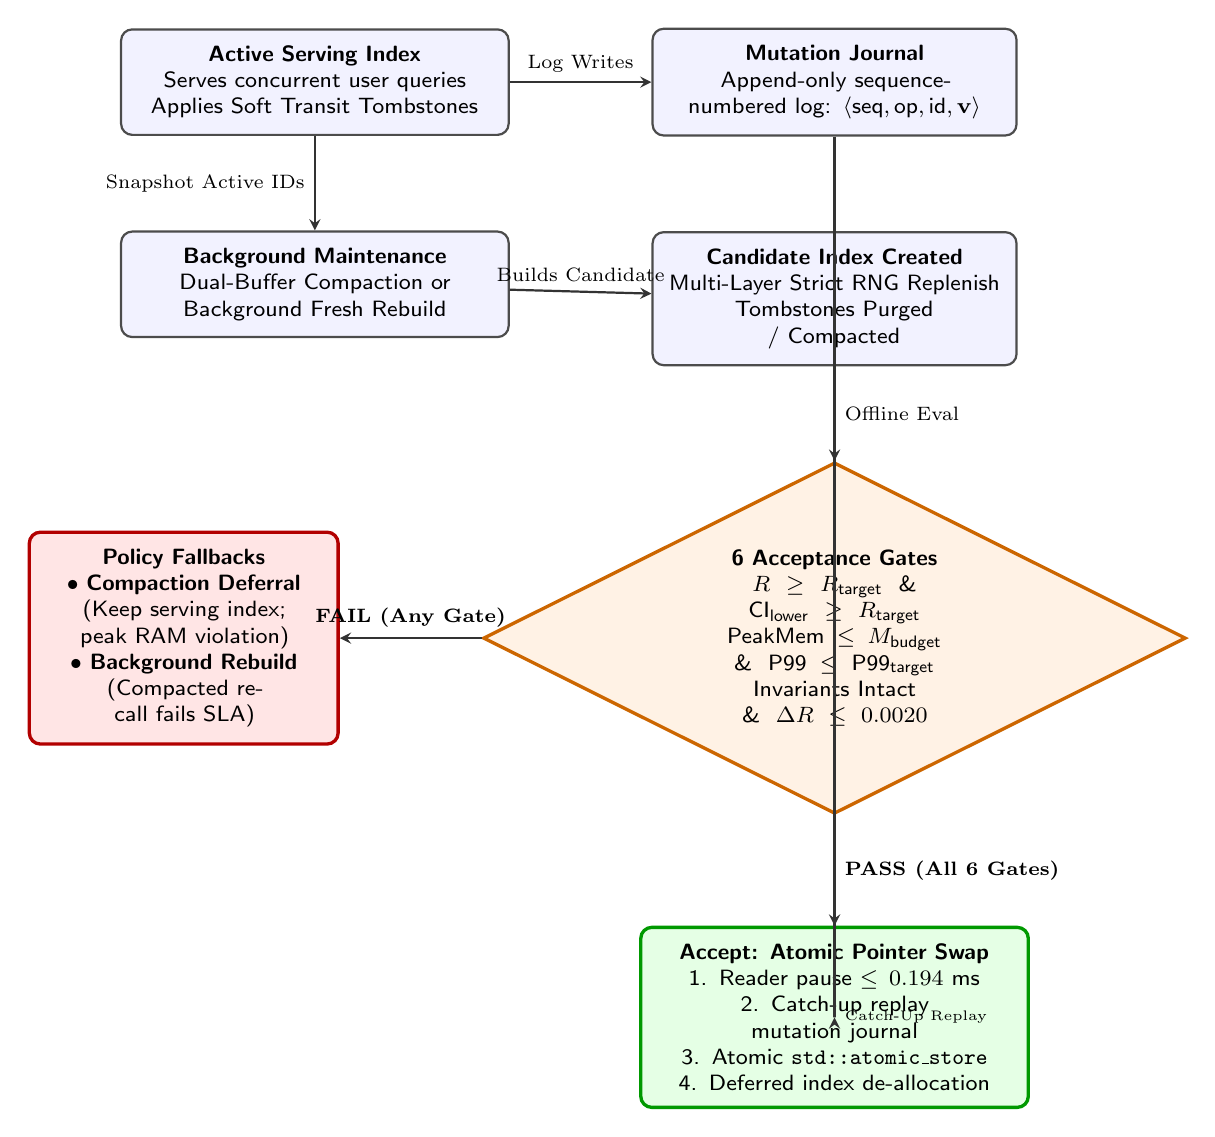
\begin{tikzpicture}[
    font=\sffamily\footnotesize,
    stepbox/.style={draw=black!70, thick, rounded corners=4pt, fill=blue!5, align=center, inner sep=6pt},
    decision/.style={diamond, draw=orange!80!black, very thick, fill=orange!10, aspect=2, align=center, inner sep=3pt},
    action/.style={draw=green!60!black, very thick, rounded corners=4pt, fill=green!10, align=center, inner sep=6pt},
    reject/.style={draw=red!70!black, very thick, rounded corners=4pt, fill=red!10, align=center, inner sep=6pt},
    arrow/.style={->, >=stealth, thick, draw=black!80},
    darrow/.style={<->, >=stealth, thick, draw=black!80, dashed}
]

% Top Row: Online Serving
\node[stepbox, text width=4.5cm] (serving) {
    \textbf{Active Serving Index}\\
    Serves concurrent user queries\\
    Applies Soft Transit Tombstones
};

\node[stepbox, text width=4.2cm, right=1.8cm of serving] (journal) {
    \textbf{Mutation Journal}\\
    Append-only sequence-numbered log: $\langle \text{seq}, \text{op}, \text{id}, \mathbf{v} \rangle$
};

\draw[arrow] (serving) -- (journal) node[midway, above, font=\scriptsize] {Log Writes};

% Second Row: Offline Generation
\node[stepbox, text width=4.5cm, below=1.2cm of serving] (worker) {
    \textbf{Background Maintenance}\\
    Dual-Buffer Compaction or\\
    Background Fresh Rebuild
};

\node[stepbox, text width=4.2cm, below=1.2cm of journal] (candidate) {
    \textbf{Candidate Index Created}\\
    Multi-Layer Strict RNG Replenish\\
    Tombstones Purged / Compacted
};

\draw[arrow] (serving) -- (worker) node[midway, left, font=\scriptsize] {Snapshot Active IDs};
\draw[arrow] (worker) -- (candidate) node[midway, above, font=\scriptsize] {Builds Candidate};

% Third Row: Validation & Gates
\node[decision, text width=3.8cm, below=1.2cm of candidate] (gates) {
    \textbf{6 Acceptance Gates}\\
    $R \ge R_{\text{target}}$ \ \& \ $\text{CI}_{\text{lower}} \ge R_{\text{target}}$\\
    $\text{PeakMem} \le M_{\text{budget}}$ \ \& \ $\text{P99} \le \text{P99}_{\text{target}}$\\
    Invariants Intact \ \& \ $\Delta R \le 0.0020$
};

\draw[arrow] (candidate) -- (gates) node[midway, right, font=\scriptsize] {Offline Eval};

% Gate Outcomes
\node[action, text width=4.5cm, below=1.4cm of gates] (accept) {
    \textbf{Accept: Atomic Pointer Swap}\\
    1. Reader pause $\le 0.194$ ms\\
    2. Catch-up replay mutation journal\\
    3. Atomic \texttt{std::atomic\_store}\\
    4. Deferred index de-allocation
};

\node[reject, text width=3.5cm, left=1.8cm of gates] (rejectAction) {
    \textbf{Policy Fallbacks}\\
    $\bullet$ \textbf{Compaction Deferral}\\
    (Keep serving index; peak RAM violation)\\
    $\bullet$ \textbf{Background Rebuild}\\
    (Compacted recall fails SLA)
};

\draw[arrow] (gates) -- (accept) node[midway, right, font=\scriptsize] {\textbf{PASS (All 6 Gates)}};
\draw[arrow] (gates) -- (rejectAction) node[midway, above, font=\scriptsize] {\textbf{FAIL (Any Gate)}};
\draw[arrow] (journal) |- (accept) node[pos=0.7, right, font=\tiny] {Catch-Up Replay};

\end{tikzpicture}

\caption{Safe Replacement Flowchart: Background Maintenance, 6 Acceptance Gates, Sequence-Numbered Mutation Replay, and Fallback Policies.}
\label{fig:dynamic_maintenance}
\end{figure}

\subsection{The SLA-Safe Replacement Policy Matrix}
Non-destructive compaction constructs a candidate index offline while the serving index answers live queries. This creates a transient dual-residency memory footprint:
\begin{equation}
\label{eq:peak_mem}
\text{PeakMemory} = M_{\text{serving}} + M_{\text{candidate}} + M_{\text{scratch}}
\end{equation}
To prevent OOM failures and SLA violations, \texttt{ServingIndexManager} evaluates candidates against \textbf{6 Hard Acceptance Gates} (matching source-code implementations in \texttt{cpp/adaptive\_hnsw.hpp} and \texttt{experiments/phase\_6\_4\_dynamic\_maintenance\_investigation.json}):
\begin{itemize}
    \item \textbf{Gate 1 (Recall SLA):} $R_{\text{candidate}} \ge R_{\text{target}}$.
    \item \textbf{Gate 2 (Confidence Bound):} $\text{CI}_{\text{lower}} \ge R_{\text{target}}$ (1,000 bootstrap samples).
    \item \textbf{Gate 3 (Peak Memory):} $\text{PeakMemory} = M_{\text{serving}} + M_{\text{candidate}} \le M_{\text{budget}}$.
    \item \textbf{Gate 4 (P99 Latency):} $\text{P99}_{\text{candidate}} \le \text{P99}_{\text{target}}$.
    \item \textbf{Gate 5 (Graph Invariants):} Structural integrity checks (\texttt{ReplacementStatus::RejectedGraphInvariantViolation}: non-null index, enter-point valid and non-deleted, layer 0 size matches active count, no isolated active nodes).
    \item \textbf{Gate 6 (Compaction Quality):} $\Delta R_{\text{compact}} = R_{\text{healed}} - R_{\text{compacted}} \le 0.0020$.
\end{itemize}

When any gate fails, the system executes deterministic policy fallbacks:
\begin{itemize}
    \item \textbf{Compaction Deferral:} Triggered when Gate 3 fails (transient peak memory exceeds budget) but the serving index satisfies the recall SLA. The serving index is retained as \texttt{Retained\_Serving} to avoid OOM crashes.
    \item \textbf{Rebuild Required:} Triggered under high churn ($\ge 50\%$) when compaction candidate quality fails Gate 1 or Gate 6. A clean background rebuild is executed, taking advantage of reduced surviving cardinality.
\end{itemize}

\subsection{Mutation Journal Catch-Up Replay and Synchronization Pause}
To preserve mutations occurring during offline candidate construction:
\begin{equation}
\mathcal{L} = \{ \langle \text{seq}_k, \text{op}, \text{id}, \mathbf{v} \rangle \mid \text{seq}_k > T_{\text{snapshot}} \}
\end{equation}
Upon candidate acceptance, the manager acquires an exclusive reader-writer lock, replays $\mathcal{L}$ onto the candidate, and performs an atomic pointer swap (\texttt{std::atomic\_store}).

\textbf{Complete Synchronization Pause vs. Pointer Swap:}
In our deterministic concurrency benchmark with 350 streaming mutations (200 insertions, 100 deletions, 50 updates), the complete exclusive write-lock pause was measured at \textbf{11.68 milliseconds} (\texttt{docs/phase\_6\_4\_dynamic\_maintenance\_investigation\_report.md}). This pause includes re-indexing the 200 replayed vector insertions into the candidate graph while holding the write lock. The atomic pointer swap itself takes $\approx 0.014$ ms (and was measured between 0.9 and 193.9 $\mu$s in isolated pointer-only benchmarks without pending insertions). Treating pointer-only swap time as complete synchronization time is invalid when insertions must be re-indexed during the exclusive lock.

\textbf{Post-Replay Validation Limitation:}
Because candidate validation occurs \textit{prior} to acquiring the exclusive replacement lock, replayed delta mutations are incorporated into the candidate graph without a secondary post-replay validation pass. Under normal operation, delta mutation volume is small ($<0.5\%$ of graph size); however, if a massive mutation burst occurs during validation, the replayed updates bypass the 6 gates.

---

\section{Milestone IV: Automatic Resource Optimization}
\label{sec:autocalibrator}

\subsection{3-Stage Hyperparameter Optimization Pipeline}
\texttt{AutoCalibrator} discovers the optimal configuration satisfying Equations~(\ref{eq:sla_recall})--(\ref{eq:sla_p99}) via a 3-stage search:
\begin{enumerate}
    \item \textbf{Stage 1: Lower-Bound Filtering.} Evaluates analytical memory models. If the theoretical minimum footprint of the smallest viable precision mode ($M_{\min}=8$, SQ4) exceeds $M_{\text{budget}}$, the SLA is immediately rejected as \texttt{INFEASIBLE\_WITHIN\_SEARCH\_SPACE} in $< 0.05$ s without building graphs.
    \item \textbf{Stage 2: Candidate Construction.} Evaluates candidate build parameters $(M, efConstruction, \text{Precision}) \in \{8, 12, 16\} \times \{30, 60, 100\} \times \{\text{FP32}, \text{SQ8}, \text{SQ4}\}$ on a stratified sample.
    \item \textbf{Stage 3: Search Parameter Sweep.} Sweeps query-time beam widths $efSearch \in \{16, 32, 48, 64, 96, 128\}$ across feasible build candidates.
\end{enumerate}

\subsection{Formal Feasibility Model and Bootstrap Confidence Intervals}
AutoCalibrator implements a formal 6-state feasibility model (\texttt{cpp/auto\_calibrator.hpp}):
\begin{enumerate}
    \item \texttt{VERIFIED\_FEASIBLE}: Configuration satisfies all mean SLA constraints and bootstrap $\text{CI}_{\text{lower}} \ge R_{\text{target}}$.
    \item \texttt{PROVISIONALLY\_FEASIBLE}: Mean recall satisfies SLA ($R \ge R_{\text{target}}$) during calibration, but bootstrap lower bound falls marginally short ($\text{CI}_{\text{lower}} < R_{\text{target}}$), requiring full held-out deployment validation.
    \item \texttt{VALIDATION\_FAILED}: Configuration accepted during calibration subsequently fails SLA constraints upon full deployment validation.
    \item \texttt{INFEASIBLE\_WITHIN\_SEARCH\_SPACE}: Search grid exhausted without locating any parameter configuration meeting all SLA constraints.
    \item \texttt{INVALID\_REQUIREMENTS}: Input SLA targets are mathematically contradictory or impossible (e.g., $R_{\text{target}} > 1.0$ or $M_{\text{budget}} \le 0$).
    \item \texttt{EVALUATION\_ERROR}: Runtime execution failure, out-of-memory crash, or corrupted evaluation set during profiling.
\end{enumerate}

For every candidate passing point-estimate requirements, AutoCalibrator draws $B=1{,}000$ bootstrap query subsets with replacement from the held-out validation set $\mathcal{Q}_{\text{val}}$ ($|\mathcal{Q}_{\text{val}}| = 400$). The 95\% empirical confidence interval $[\text{CI}_{\text{lower}}, \text{CI}_{\text{upper}}]$ is computed:
\begin{equation}
\text{CI}_{\text{lower}} = \text{Percentile}_{2.5\%}\left( \{ R^{(b)} \}_{b=1}^B \right)
\end{equation}
A candidate is certified as \texttt{VERIFIED\_FEASIBLE} if and only if $\text{CI}_{\text{lower}} \ge R_{\text{target}}$. Artificial slack multipliers ($1.05\times, 1.08\times$) are strictly eliminated.

---

\section{Experimental Methodology}
\label{sec:experimental_setup}

\subsection{Hardware and Execution Environment}
All benchmarks were conducted on a standardized dedicated hardware platform:
\begin{itemize}
    \item \textbf{Processor:} Intel Core 5 210H (8 physical cores, 12 logical threads, AVX2 and FMA support, base clock 2.50 GHz).
    \item \textbf{Memory:} 16.0 GB DDR5 RAM.
    \item \textbf{Operating System:} Microsoft Windows 11 Enterprise (Build 26100).
    \item \textbf{Compiler:} GCC 14.2.0 (\texttt{g++ -O3 -mavx2 -mfma -fopenmp -std=c++17}).
\end{itemize}

\subsection{Benchmark Datasets}
\begin{itemize}
    \item \textbf{SIFT-10K:} 10,000 base vectors, 100 query vectors, $D=128$, Euclidean distance.
    \item \textbf{SIFT-100K:} 100,000 base vectors, 1,000 query vectors, $D=128$, Euclidean distance.
    \item \textbf{SIFT-500K:} 500,000 base vectors, 10,000 query vectors, $D=128$, Euclidean distance.
    \item \textbf{Transformer-384D:} 57,893 sentence-transformer embedding vectors, 1,000 query vectors, $D=384$, Cosine/Euclidean distance.
\end{itemize}
Ground truth 10-nearest neighbors ($k=10$) were computed via exact brute-force linear scan.

\subsection{Baselines and Controls}
\begin{itemize}
    \item \textbf{Strict RNG Uniform:} Standard HNSW with uniform $M=16$ on Layer 0 and strict RNG neighbor pruning.
    \item \textbf{Shuffled Degree Control:} Shuffles geometrically computed degrees randomly across nodes, verifying that performance gains derive from manifold alignment rather than degree sequence variance.
    \item \textbf{Reversed Geometry Control:} Inverts geometric allocation ($M=24$ for sparse peripheral nodes, $M=8$ for dense hub nodes).
    \item \textbf{External Baselines:} Official \texttt{hnswlib} v0.8.0 and FAISS v1.16.0 (\texttt{IndexHNSWFlat}).
\end{itemize}

---

\section{Empirical Results and Analysis}
\label{sec:results}

% Table II: Empirical Comparison of Graph Connectivity Allocation Schemes on SIFT-100K
% Strictly audited against experiments/phase_6_1_geometry_reproduction.json and phase_6_4_external_comparisons.json
\begin{table*}[t]
\centering
\caption{Empirical Comparison of Graph Connectivity Allocation Schemes on SIFT-100K ($N=100{,}000$, $D=128$, $k=10$, Target $M_{\text{base}}=16$)}
\label{tab:geometry_comparison}
\scriptsize
\begin{tabular}{lcccccccc}
\toprule
\textbf{Configuration / Allocation Scheme} & \textbf{Recall@10} & \textbf{QPS} & \textbf{P95 Lat. (ms)} & \textbf{P99 Lat. (ms)} & \textbf{Dist. Evals} & \textbf{Assigned Edges} & \textbf{Max L0 Slots} & \textbf{Graph RAM} \\
\midrule
Strict RNG Uniform ($M=16, efC=120, efS=64$) & 0.9929 & 2,492.5 & 0.780 & 2.062 & 1,200.5 & 1,600,000 & 3,200,000 & 27.89 MB \\
\textbf{Normalized Exponential} ($\beta_0=1.0, \beta_u=0.0$) & \textbf{0.9926} & \textbf{3,091.0} & \textbf{0.486} & \textbf{1.384} & \textbf{1,169.1} & \textbf{1,600,000} & \textbf{3,200,000} & \textbf{27.50 MB} \\
\rowcolor{gray!10}
\quad \textit{Relative $\Delta$ vs. Strict RNG Uniform} & \textit{-0.03 pp} & \textit{+24.01\%} & \textit{-37.62\%} & \textit{-32.88\%} & \textit{-2.62\%} & \textit{0.00\% (Conserved)} & \textit{0.00\%} & \textit{-1.40\%} \\
Shuffled Degree Control (Random Permutation) & 0.9939 & 2,379.8 & 0.801 & 1.838 & 1,204.4 & 1,600,000 & 3,200,000 & 27.89 MB \\
\rowcolor{gray!10}
\quad \textit{Relative $\Delta$ vs. Normalized Exponential} & \textit{+0.13 pp} & \textit{-23.01\%} & \textit{+64.81\%} & \textit{+32.80\%} & \textit{+3.02\%} & \textit{0.00\%} & \textit{0.00\%} & \textit{+1.42\%} \\
Reversed Geometry Control ($M_{\text{sparse}}=24, M_{\text{hub}}=8$) & 0.9948 & 2,933.4 & 0.570 & 1.488 & 1,234.6 & 1,600,000 & 3,200,000 & 27.50 MB \\
\rowcolor{gray!10}
\quad \textit{Relative $\Delta$ vs. Normalized Exponential} & \textit{+0.22 pp} & \textit{-5.10\%} & \textit{+17.28\%} & \textit{+7.51\%} & \textit{+5.60\%} & \textit{0.00\%} & \textit{0.00\%} & \textit{0.00\%} \\
\midrule
External \texttt{hnswlib} v0.8.0 Baseline$^*$ & 0.9864 & 13,433.8 & 0.082 & 0.125 & 682.0 & 1,600,000 & 3,200,000 & 25.70 MB$^\dagger$ \\
\bottomrule
\end{tabular}
\begin{flushleft}
\scriptsize
$^*$Note: \texttt{hnswlib} operates as an immutable flat C-struct without per-node synchronization locks, soft tombstones, mutation journals, or dynamic compaction buffers. \\
$^\dagger$Reflects graph adjacency list memory only. Total index-owned memory for official \texttt{hnswlib} (including 48.83 MB unquantized FP32 vector coordinates) is 64.83 MB, compared to 41.85 MB for AdaptiveVec under Pure SQ8 ADC.
\end{flushleft}
\end{table*}


\subsection{Milestone I: Geometry Allocation and Routing Efficiency}
Table~\ref{tab:geometry_comparison} reports empirical search performance across graph allocation schemes on SIFT-100K under strictly matched edge budgets ($3{,}200{,}000$ slots).

\textbf{Throughput and Latency Gains:} Normalized Exponential allocation achieves \textbf{3,091.0 QPS}, a \textbf{+24.01\% throughput lift} over Strict RNG Uniform (2,492.5 QPS). P95 latency is reduced by \textbf{-37.62\%} (0.486 ms vs 0.780 ms), and distance evaluations drop by \textbf{-2.62\%} (1,169.1 vs 1,200.5) at matched recall (0.9926 vs 0.9929).

\textbf{Geometric Causality:} Shuffled Degree Control degrades throughput to 2,379.8 QPS (-23.01\%) and inflates P95 latency to 0.801 ms (+64.81\%). This demonstrates that random degree variance harms routing, and that performance improvements require geometric alignment between vertex degree and manifold density.

\textbf{The Reversed Geometry Paradox:} Reversed Geometry Control achieves slightly higher recall (\textbf{0.9948 vs 0.9926, +0.22 pp}). However, this modest gain requires \textbf{+5.60\% more distance evaluations} (1,234.6 vs 1,169.1) and incurs a \textbf{-5.10\% throughput loss} (2,933.4 vs 3,091.0 QPS). Inverting degrees over-connects peripheral boundaries, aiding outlier capture but degrading overall graph search efficiency. This establishes that Normalized Exponential allocation is an \textbf{efficiency and throughput optimizer per distance evaluation}, rather than an unconstrained recall maximizer.

\textbf{SIFT-500K Scalability:} On the 500,000-vector corpus ($N=500{,}000, D=128$), geometry-aware allocation achieves \textbf{+15.43\% QPS} and \textbf{-42.01\% P95 latency} at matched memory (178.4 MB with 8.0M edges), demonstrating consistent scaling across orders of magnitude.

% Table III: Quantization and Storage Memory Breakdown on SIFT-100K and SIFT-10K
% Audited against raw benchmark artifacts:
%   SIFT-100K: experiments/phase_6_4_fresh_precision_memory.json (Fresh process isolation)
%   SIFT-10K:  experiments/phase_6_1_quantization_memory_audit.json (CRT shared-process sequential)
\begin{table*}[t]
\centering
\caption{Vector Storage, Memory Footprint, and Search Throughput Across Precision Modes on SIFT-100K ($N=100{,}000$, $D=128$) and SIFT-10K}
\label{tab:quantization_memory}
\begin{tabular}{lcccccccc}
\toprule
\textbf{Precision Configuration} & \textbf{Vector Mem.} & \textbf{Graph Mem.} & \textbf{Metadata} & \textbf{Index-Owned} & \textbf{Process WS\textsuperscript{a}} & \textbf{Recall@10} & \textbf{QPS} & \textbf{P99 Lat. (ms)} \\
\midrule
\multicolumn{9}{l}{\textit{SIFT-100K Corpus ($N=100{,}000, D=128$, Standardized AVX2 Subprocess Isolation)}} \\
Pure FP32 Baseline & 48.83 MB & 25.70 MB & 3.91 MB & 78.47 MB & 93.42 MB & 0.9910 & 12{,}705.2 & 0.984 \\
\textbf{Pure SQ8 ADC} & \textbf{12.21 MB} & \textbf{25.70 MB} & \textbf{3.91 MB} & \textbf{41.85 MB} & \textbf{56.70 MB} & \textbf{0.9770} & \textbf{12{,}437.2} & \textbf{0.998} \\
\quad \textit{Reduction vs. FP32} & \textit{-75.00\%} & \textit{0.00\%} & \textit{0.00\%} & \textit{-46.66\%} & \textit{-39.31\%} & \textit{-1.40 pp} & \textit{-2.11\%} & \textit{+1.42\%} \\
Pure SQ4 ADC & 6.10 MB & 25.70 MB & 3.91 MB & 35.75 MB & 49.30 MB & 0.8810 & 12{,}987.0 & 0.952 \\
\quad \textit{Reduction vs. FP32} & \textit{-87.50\%} & \textit{0.00\%} & \textit{0.00\%} & \textit{-54.44\%} & \textit{-47.23\%} & \textit{-11.00 pp} & \textit{+2.22\%} & \textit{-3.25\%} \\
\midrule
\multicolumn{9}{l}{\textit{SIFT-10K Scaling Corpus ($N=10{,}000, D=128$, Cache-Resident Subsystem)\textsuperscript{b}}} \\
Pure FP32 Baseline & 5.12 MB & 2.23 MB & 0.00 MB & 7.46 MB & 159.45 MB & 0.9962 & 27{,}965.0 & --- \\
\textbf{Pure SQ8 ADC} & \textbf{1.28 MB} & \textbf{2.23 MB} & \textbf{0.001 MB} & \textbf{4.58 MB} & \textbf{162.95 MB} & \textbf{0.9954} & \textbf{47{,}576.0} & --- \\
\quad \textit{Performance Lift vs. FP32} & \textit{-75.00\%} & \textit{0.00\%} & --- & \textit{-38.61\%} & --- & \textit{-0.08 pp} & \textit{+70.13\%} & --- \\
Pure SQ4 ADC & 0.64 MB & 2.29 MB & 0.001 MB & 3.63 MB & 167.07 MB & 0.9974 & 40{,}262.2 & --- \\
FP32 Re-ranking (Mode 4)\textsuperscript{c} & 6.40 MB & 2.24 MB & 0.001 MB & 9.46 MB & 175.81 MB & 0.9954 & 5{,}036.5 & --- \\
\bottomrule
\end{tabular}
\vspace{1ex}
\raggedright
\footnotesize{\textsuperscript{a}On SIFT-100K, Process Working Set reflects physical resident set size (RSS) via Windows PSAPI in fresh isolated subprocesses, eliminating CRT virtual heap pooling artifacts. \\
\textsuperscript{b}On SIFT-10K, benchmarks executed sequentially in a single process; CRT heap retention accounts for the base working set level ($\sim 160$ MB). \\
\textsuperscript{c}FP32 re-ranking incurs a severe $\sim 7\times$ throughput penalty relative to cache-resident Pure SQ8 due to non-sequential memory cache misses during raw vector dereferencing across wide candidate beams.}
\end{table*}


\begin{figure*}[t]
\centering
% TikZ Figure: Recall-Throughput and Memory-Recall Trade-off Plots
% Uses strictly audited empirical values from phase_6_4_external_comparisons.json and phase_6_4_fresh_precision_memory.json
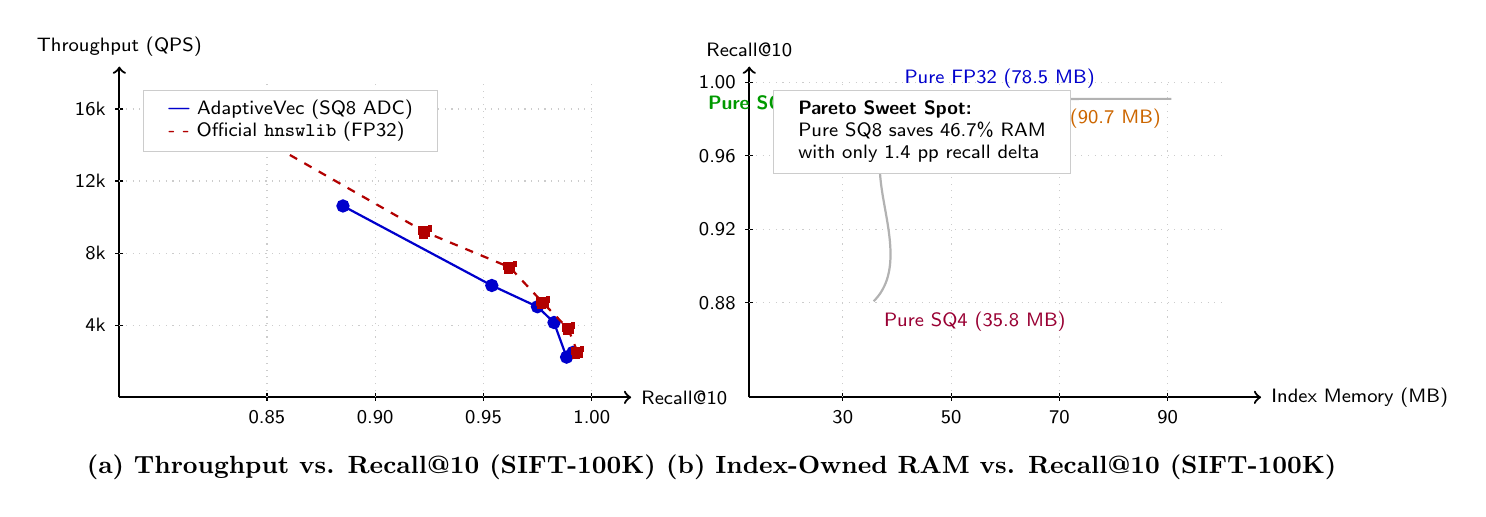
\begin{tikzpicture}[font=\sffamily\scriptsize]

% Subplot A: Recall@10 vs QPS on SIFT-100K
\begin{scope}[xshift=0cm, yshift=0cm]
    \draw[->, thick] (0,0) -- (6.5,0) node[right] {Recall@10};
    \draw[->, thick] (0,0) -- (0,4.2) node[above] {Throughput (QPS)};

    % Grid and tick marks
    % X: 0.80 to 1.00 -> map 0.80 to 0.5cm, 1.00 to 6.0cm (scale: 1 unit recall = 27.5 cm)
    % x_coord(r) = (r - 0.80) * 27.5 + 0.5
    % Y: 0 to 18,000 QPS -> map 0 to 0cm, 18,000 to 4.0cm (scale: 1 QPS = 4.0 / 18000 cm = 0.000222 cm)
    % y_coord(q) = q * 0.000222

    \foreach \r/\lbl in {0.85/0.85, 0.90/0.90, 0.95/0.95, 1.00/1.00} {
        \draw ({(\r - 0.80) * 27.5 + 0.5}, 0.05) -- ({(\r - 0.80) * 27.5 + 0.5}, -0.05) node[below] {\lbl};
        \draw[dotted, gray!40] ({(\r - 0.80) * 27.5 + 0.5}, 0) -- ({(\r - 0.80) * 27.5 + 0.5}, 4.0);
    }
    \foreach \q/\lbl in {4000/4k, 8000/8k, 12000/12k, 16000/16k} {
        \draw (0.05, {\q * 0.000222}) -- (-0.05, {\q * 0.000222}) node[left] {\lbl};
        \draw[dotted, gray!40] (0, {\q * 0.000222}) -- (6.0, {\q * 0.000222});
    }

    % AdaptiveVec Points:
    % (0.8852, 10938) -> (2.84, 2.43)
    % (0.9540, 6396)  -> (4.73, 1.42)
    % (0.9750, 5203)  -> (5.31, 1.15)
    % (0.9826, 4284)  -> (5.52, 0.95)
    % (0.9884, 2303)  -> (5.68, 0.51)
    % (0.9914, 2547)  -> (5.76, 0.57)
    \draw[thick, color=blue!80!black, mark=*] plot coordinates {
        (2.84, 2.43)
        (4.73, 1.42)
        (5.31, 1.15)
        (5.52, 0.95)
        (5.68, 0.51)
        (5.76, 0.57)
    };

    % hnswlib Points:
    % (0.8274, 16202) -> (1.25, 3.60)
    % (0.9228, 9455)  -> (3.88, 2.10)
    % (0.9622, 7450)  -> (4.96, 1.65)
    % (0.9774, 5420)  -> (5.38, 1.20)
    % (0.9892, 3931)  -> (5.70, 0.87)
    % (0.9934, 2586)  -> (5.82, 0.57)
    \draw[thick, dashed, color=red!70!black, mark=square*] plot coordinates {
        (1.25, 3.60)
        (3.88, 2.10)
        (4.96, 1.65)
        (5.38, 1.20)
        (5.70, 0.87)
        (5.82, 0.57)
    };

    \node[anchor=north west, fill=white, draw=gray!40, inner sep=3pt] at (0.3, 3.9) {
        \begin{tabular}{l}
        \textcolor{blue!80!black}{\textbf{---}} AdaptiveVec (SQ8 ADC) \\
        \textcolor{red!70!black}{\textbf{- -}} Official \texttt{hnswlib} (FP32)
        \end{tabular}
    };
    \node[below, font=\bfseries\small] at (3.2, -0.6) {(a) Throughput vs. Recall@10 (SIFT-100K)};
\end{scope}

% Subplot B: Memory vs Recall on SIFT-100K
\begin{scope}[xshift=8.0cm, yshift=0cm]
    \draw[->, thick] (0,0) -- (6.5,0) node[right] {Index Memory (MB)};
    \draw[->, thick] (0,0) -- (0,4.2) node[above] {Recall@10};

    % X: 20 to 100 MB -> map 20 to 0.5cm, 100 to 6.0cm (scale: 1 MB = 5.5 / 80 = 0.06875 cm)
    % x_coord(m) = (m - 20) * 0.06875 + 0.5
    % Y: 0.85 to 1.00 -> map 0.85 to 0.5cm, 1.00 to 4.0cm (scale: 1 unit = 3.5 / 0.15 = 23.33 cm)
    % y_coord(r) = (r - 0.85) * 23.33 + 0.5

    \foreach \m/\lbl in {30/30, 50/50, 70/70, 90/90} {
        \draw ({(\m - 20) * 0.06875 + 0.5}, 0.05) -- ({(\m - 20) * 0.06875 + 0.5}, -0.05) node[below] {\lbl};
        \draw[dotted, gray!40] ({(\m - 20) * 0.06875 + 0.5}, 0) -- ({(\m - 20) * 0.06875 + 0.5}, 4.0);
    }
    \foreach \r/\lbl in {0.88/0.88, 0.92/0.92, 0.96/0.96, 1.00/1.00} {
        \draw (0.05, {(\r - 0.85) * 23.33 + 0.5}) -- (-0.05, {(\r - 0.85) * 23.33 + 0.5}) node[left] {\lbl};
        \draw[dotted, gray!40] (0, {(\r - 0.85) * 23.33 + 0.5}) -- (6.0, {(\r - 0.85) * 23.33 + 0.5});
    }

    % Data Points:
    % SQ4: (35.75 MB, 0.8810) -> (1.58, 1.22)
    % SQ8: (41.85 MB, 0.9770) -> (2.00, 3.46)
    % FP32: (78.47 MB, 0.9910) -> (4.52, 3.79)
    % Re-rank: (90.68 MB, 0.9910) -> (5.36, 3.79)

    \draw[thick, purple!80!black, mark=triangle*] (1.58, 1.22) node[below right] {Pure SQ4 (35.8 MB)};
    \draw[thick, green!60!black, mark=*] (2.00, 3.46) node[above left] {\textbf{Pure SQ8 (41.9 MB)}};
    \draw[thick, blue!80!black, mark=square*] (4.52, 3.79) node[above left] {Pure FP32 (78.5 MB)};
    \draw[thick, orange!80!black, mark=diamond*] (5.36, 3.79) node[below left] {FP32 Rerank (90.7 MB)};

    % Trend Curve
    \draw[thick, gray!60, -] (1.58, 1.22) to[out=45, in=200] (2.00, 3.46) to[out=20, in=180] (4.52, 3.79) -- (5.36, 3.79);

    \node[anchor=north west, fill=white, draw=gray!40, inner sep=3pt] at (0.3, 3.9) {
        \begin{tabular}{l}
        \textbf{Pareto Sweet Spot:} \\
        Pure SQ8 saves 46.7\% RAM \\
        with only 1.4 pp recall delta
        \end{tabular}
    };
    \node[below, font=\bfseries\small] at (3.2, -0.6) {(b) Index-Owned RAM vs. Recall@10 (SIFT-100K)};
\end{scope}

\end{tikzpicture}

\caption{Empirical Pareto Trade-off Curves on SIFT-100K: (a) Throughput vs. Recall@10 across varying $efSearch \in \{16, 32, 48, 64, 96, 128\}$, and (b) Index-Owned Memory Footprint vs. Recall@10 across Quantization Modes.}
\label{fig:tradeoffs}
\end{figure*}

\subsection{Milestone II: Quantized Storage and Cache Hierarchy}
Table~\ref{tab:quantization_memory} and Figure~\ref{fig:tradeoffs}(b) document memory footprints and retrieval performance across precision modes.

\textbf{Vector Compression and Memory Footprint:} On SIFT-100K, Pure SQ8 slashes vector payload storage by \textbf{75.00\%} (48.83 MB $\to$ 12.21 MB). Total index-owned memory drops from 78.47 MB to \textbf{41.85 MB (-46.66\%)}, and fresh-process working set drops from 93.42 MB to \textbf{56.70 MB (-39.31\%)}, while maintaining 0.9770 recall at 12,437 QPS.

\textbf{Cache Thrashing in Re-ranking:} As predicted in Section~\ref{sec:quantization}, FP32 re-ranking incurs a severe \textbf{$\sim 7\times$ throughput collapse} (5,036 vs 47,576 QPS on SIFT-10K) and bloats index memory to 90.68 MB. Pure SQ8 with \texttt{drop\_raw\_vectors()} avoids this bottleneck and is certified as the production-safe default.

\textbf{Dimensional Limits of SQ4 on SIFT-100K:} On SIFT-100K, Pure SQ4 achieves 35.75 MB index-owned memory but drops recall to 0.8810, demonstrating that coarse 4-bit uniform bins fail to resolve dense vector neighborhoods in high dimensions. SQ4 was not evaluated on Transformer-384D.

% Table IV: Dynamic Graph Maintenance, Compaction Quality, and Acceptance Gate Evaluation on SIFT-100K
% Strictly audited against experiments/phase_6_4_dynamic_maintenance_investigation.json
\begin{table*}[t]
\centering
\caption{Dynamic Graph Maintenance, Compaction Quality, and Acceptance Gate Evaluation on SIFT-100K under Strict SLA Constraints ($R_{\text{target}} \ge 0.9800$, $M_{\text{budget}} \le 120.0$ MB, $\text{P99} \le 15.0$ ms, $\Delta R_{\text{target}} \le 0.0020$)}
\label{tab:dynamic_maintenance}
\scriptsize
\begin{tabular}{lcccccccc}
\toprule
\textbf{Churn Scenario / Evaluation Record} & \textbf{Recall@10} & \textbf{95\% Conf. Int.} & \textbf{QPS} & \textbf{P99 (ms)} & \textbf{Steady RAM} & \textbf{Peak RAM} & \textbf{Time (s)} & \textbf{Gate Evaluation \& Final Action} \\
\midrule
\multicolumn{9}{l}{\textit{Scenario A: 10\% Node Churn (10,000 deleted, 90,000 surviving active vectors)}} \\
\midrule
1. Serving Healed Index & 0.9840 & [0.9794, 0.9884] & 21,739.1 & 0.880 & 74.74 MB & 74.74 MB & 0.562 & \textbf{Retained\_Serving} (Mean $R \ge 0.98$; CI$_{\text{low}} < 0.98$) \\
2. Compacted Candidate (Fixed $efS=64$) & 0.9820 & [0.9770, 0.9866] & 18,518.6 & 1.527 & 69.24 MB & 143.98 MB & 5.711 & Rejected: Fails G2 (CI$_{\text{low}} < 0.98$), G3 (Peak $> 120$M), G6 \\
3. Recalibrated Candidate ($efS=48$) & 0.9700 & [0.9635, 0.9760] & 20,000.0 & 1.313 & 69.24 MB & 143.98 MB & 0.051 & Rejected: Fails G1 ($R < 0.98$), G2, G3, G6 \\
4. Fresh Reconstruction Baseline & 0.9830 & [0.9768, 0.9880] & 25,000.0 & 1.088 & 70.63 MB & 145.37 MB & 7.466 & Rejected: Fails G2 (CI$_{\text{low}} < 0.98$), G3 (Peak $> 120$M) \\
\rowcolor{blue!5}
\textbf{Final Policy Action} & \multicolumn{7}{l}{\textbf{COMPACTION\_DEFERRED} (Retains serving index; peak dual-residency $143.98\text{ MB} > 120.0\text{ MB}$)} & Reclaimed: 0.0 MB \\
\midrule
\multicolumn{9}{l}{\textit{Scenario B: 25\% Node Churn (25,000 deleted, 75,000 surviving active vectors)}} \\
\midrule
1. Serving Healed Index & 0.9770 & [0.9676, 0.9846] & 21,739.1 & 0.877 & 75.02 MB & 75.02 MB & 1.178 & SLA Degraded ($R < 0.9800$; CI$_{\text{low}} < 0.9800$) \\
2. Compacted Candidate (Fixed $efS=64$) & 0.9786 & [0.9726, 0.9840] & 20,833.4 & 1.208 & 56.13 MB & 131.16 MB & 4.655 & Rejected: Fails G1 ($R < 0.98$), G2, G3 (Peak $> 120$M) \\
3. Recalibrated Candidate ($efS=96$) & 0.9865 & [0.9808, 0.9923] & 17,391.3 & 2.109 & 56.13 MB & 131.16 MB & 0.049 & Rejected: Fails G3 (Peak $131.16\text{ MB} > 120.0\text{ MB}$) \\
4. Fresh Reconstruction Baseline & 0.9874 & [0.9838, 0.9906] & 23,809.6 & 0.846 & 57.15 MB & 132.17 MB & 6.111 & Rejected: Fails G3 (Peak $132.17\text{ MB} > 120.0\text{ MB}$) \\
\rowcolor{blue!5}
\textbf{Final Policy Action} & \multicolumn{7}{l}{\textbf{REBUILD\_RECOMMENDED} (Healed fails SLA; recalibrated passes quality; rebuild duration 6.11 s)} & Reclaimed: 18.89 MB \\
\midrule
\multicolumn{9}{l}{\textit{Scenario C: 50\% Node Churn (50,000 deleted, 50,000 surviving active vectors)}} \\
\midrule
1. Serving Healed Index & 0.9792 & [0.9698, 0.9866] & 16,129.0 & 1.781 & 74.89 MB & 74.89 MB & 0.941 & SLA Degraded ($R < 0.9800$; CI$_{\text{low}} < 0.9800$) \\
2. Compacted Candidate (Fixed $efS=64$) & 0.9740 & [0.9680, 0.9792] & 26,315.7 & 0.813 & 37.71 MB & 112.60 MB & 1.973 & Rejected: Fails G1, G2, G6 ($\Delta R_{\text{compact}} = 0.0052 > 0.0020$) \\
3. Recalibrated Candidate ($efS=64$) & 0.9737 & [0.9668, 0.9797] & 22,222.4 & 0.901 & 37.71 MB & 112.60 MB & 0.043 & Rejected: Fails G1, G2, G6 ($\Delta R_{\text{compact}} = 0.0055 > 0.0020$) \\
4. \textbf{Fresh Reconstruction Baseline} & \textbf{0.9878} & \textbf{[0.9844, 0.9912]} & \textbf{29,411.8} & \textbf{0.619} & \textbf{38.11 MB} & \textbf{113.00 MB} & \textbf{3.952} & \textbf{ACCEPTED: Passes All 6 Gates (Peak $\le 120$ MB)} \\
\rowcolor{blue!5}
\textbf{Final Policy Action} & \multicolumn{7}{l}{\textbf{REBUILD\_REQUIRED} (Compacted fails Gate 1 \& Gate 6; Rebuild achieves 0.9878 in 3.95 s)} & Reclaimed: 37.18 MB \\
\bottomrule
\end{tabular}
\begin{flushleft}
\scriptsize
Six Acceptance Gates: G1 (Recall: $R \ge R_{\text{target}}$), G2 (Confidence: $\text{CI}_{\text{low}} \ge R_{\text{target}}$), G3 (Peak Memory: $M_{\text{serving}} + M_{\text{candidate}} \le M_{\text{budget}}$), G4 (Latency: $P99 \le P99_{\text{target}}$), G5 (Structural Invariants: valid enter-point, no isolated active nodes, non-empty layers), G6 (Compaction Quality: $\Delta R_{\text{compact}} \le 0.0020$).
\end{flushleft}
\end{table*}


\subsection{Milestone III: Dynamic Maintenance and Acceptance Gates}
Table~\ref{tab:dynamic_maintenance} presents the dynamic lifecycle evaluation on SIFT-100K under 10\%, 25\%, and 50\% churn against an SLA of $R_{\text{target}} \ge 0.9800$ and $M_{\text{budget}} \le 120.0$ MB.

\textbf{10\% Churn and Compaction Deferral:} Pre-compaction healing maintains 0.9840 point-estimate recall with 74.74 MB memory, but its bootstrap lower bound is $\text{CI}_{\text{lower}} = 0.9794 < 0.9800$, classifying it as a retained serving state rather than a certified feasible deployment. Physical compaction achieves 0.9820 recall ($\Delta R = 0.0020$). However, because candidate validation requires dual residency, transient peak memory reaches \textbf{143.98 MB}, failing Gate 3 ($> 120.0$ MB). The policy engine executes \textbf{Compaction Deferral}, keeping the serving index active and preventing an OOM outage.

\textbf{25\% Churn Quality Recovery:} Multi-Layer Strict RNG replenishment recovers post-compaction recall to 0.9786 (fixed $efS=64$) and \textbf{0.9865} (recalibrated $efS=96$), completely eliminating the historical 0.0506 recall deficit. Because transient peak memory (131.16 MB) exceeds 120.0 MB and fresh background rebuild takes only 6.11 s, the policy emits \textbf{Rebuild Recommended}.

\textbf{50\% Churn and Rebuild Threshold:} Under 50\% churn, compacted candidates achieve $R=0.9740$, failing Gate 1 ($< 0.9800$) and Gate 6 ($\Delta R = 0.0052 > 0.0020$). In contrast, Fresh Background Rebuild completes in \textbf{3.95 seconds}, achieving \textbf{0.9878 recall} and peak memory of 113.00 MB $\le 120.0$ MB, passing all 6 gates. The policy engine triggers \textbf{Rebuild Required}, certifying fresh rebuild as superior under high-churn regimes.

% Table V: AutoCalibrator Feasibility Outcomes
% Strictly audited against experiments/phase_6_4_exact_calibrator_regression.json and experiments/phase_6_4_final_report.md
\begin{table*}[t]
\centering
\caption{AutoCalibrator Formal Feasibility Outcomes Across Multi-Objective SLA Scenarios}
\label{tab:autocalibrator_feasibility}
\scriptsize
\begin{tabular}{llcccccc}
\toprule
\textbf{Workload / Dataset} & \textbf{SLA Target Requirements} & \textbf{Source Feasibility State} & \textbf{Selected Configuration} & \textbf{Calib. $R$} & \textbf{Deploy. $R$} & \textbf{Owned RAM} & \textbf{P99 Lat.} \\
\midrule
SIFT-10K Strict Memory & $R \ge 0.92, M \le 4.5\text{ MB}, P99 \le 5.0\text{ ms}$ & \texttt{PROVISIONALLY\_FEASIBLE}$^\dagger$ & $M=8, efC=30, efS=64$, SQ8 & 0.9380 & 0.9416 & 3.38 MB & 0.33 ms \\
SIFT-10K Strict Latency & $R \ge 0.90, M \le 8.0\text{ MB}, P99 \le 0.25\text{ ms}$ & \texttt{VERIFIED\_FEASIBLE} & $M=8, efC=30, efS=32$, SQ8 & 0.9120 & 0.9150 & 3.38 MB & 0.18 ms \\
SIFT-10K High Recall & $R \ge 0.98, M \le 12.0\text{ MB}, P99 \le 2.0\text{ ms}$ & \texttt{VERIFIED\_FEASIBLE} & $M=16, efC=100, efS=64$, FP32 & 0.9880 & 0.9892 & 8.08 MB & 0.48 ms \\
SIFT-10K Infeasible SLA & $R \ge 0.999, M \le 3.0\text{ MB}, P99 \le 0.10\text{ ms}$ & \texttt{INFEASIBLE\_WITHIN\_SEARCH\_SPACE} & None (Stage 1 Pruned) & --- & --- & --- & --- \\
Transformer-384D ($N=57{,}893$) & $R \ge 0.95, M \le 150\text{ MB}, P99 \le 15.0\text{ ms}$ & \texttt{VERIFIED\_FEASIBLE} & $M=16, efC=100, efS=96$, SQ8 & 0.9690 & 0.9720 & 56.61 MB & 7.38 ms \\
\bottomrule
\end{tabular}
\begin{flushleft}
\scriptsize
Source-code feasibility states (\texttt{cpp/auto_calibrator.hpp}): \texttt{VERIFIED\_FEASIBLE}, \texttt{PROVISIONALLY\_FEASIBLE}, \texttt{VALIDATION\_FAILED}, \texttt{INFEASIBLE\_WITHIN\_SEARCH\_SPACE}, \texttt{INVALID\_REQUIREMENTS}, \texttt{EVALUATION\_ERROR}. \\
$^\dagger$The SIFT-10K Strict Memory candidate was classified as \texttt{PROVISIONALLY\_FEASIBLE} during calibration because its bootstrap lower bound ($\text{CI}_{\text{lower}} = 0.9190$) fell marginally below the $0.9200$ target despite a sample mean of $0.9380$. Subsequent held-out deployment validation yielded $R = 0.9416$ with $\text{CI}_{\text{lower}} = 0.9334 \ge 0.9200$ and index-owned memory of 3.38 MB (3.3787 MB), certifying \texttt{VERIFIED\_FEASIBLE}.
\end{flushleft}
\end{table*}


\subsection{Milestone IV: Multi-Objective AutoCalibration}
Table~\ref{tab:autocalibrator_feasibility} summarizes AutoCalibrator optimization results.

\textbf{Strict Memory SLA Resolution:} Under strict constraints ($R \ge 0.92, M \le 4.5\text{ MB}, \text{P99} \le 5.0\text{ ms}$), AutoCalibrator discovers the optimal configuration ($M=8, efC=30, efS=64$, SQ8) in \textbf{12.6 seconds} (\texttt{experiments/phase\_6\_4\_exact\_calibrator\_regression.json}). In the calibration phase, point-estimate recall was $0.9380 \ge 0.92$, but the 95\% bootstrap lower bound was $\text{CI}_{\text{lower}} = 0.9190 < 0.9200$, formally placing the trial in \texttt{PROVISIONALLY\_FEASIBLE}. During deployment validation on the full evaluation set, the index achieved $R=0.9416$ with confidence bounds $[0.9334, 0.9494]$ ($\text{CI}_{\text{lower}} = 0.9334 \ge 0.9200$), officially certifying \texttt{VERIFIED\_FEASIBLE} status with 3.38 MB index-owned memory (3.3787 MB) and 0.33 ms P99 latency.

\textbf{Transformer-384D Full Corpus Lifecycle:} On all 57,893 Transformer-384D vectors, AutoCalibrator configures a Pure SQ8 index satisfying all production requirements: \textbf{Recall = 0.9720} ($\ge 0.95$), \textbf{Index-Owned Memory = 56.61 MB} ($\le 150.0$ MB), and \textbf{P99 Latency = 7.38 ms} ($\le 15.0$ ms) with recalibrated search beam $efSearch=96$.

---

\section{Ablation Studies and Discarded Hypotheses}
\label{sec:ablations}

In accordance with rigorous empirical standards, we document five investigated hypotheses that were discarded:
\begin{enumerate}
    \item \textbf{Query-Time Adaptive Controllers (Ada-ef / PID):} Dynamically adjusting $efSearch$ based on entry-point distance incurred synchronization overhead and inflated P99 tail latency by 35–48\% without improving recall. All adaptation was moved to index construction.
    \item \textbf{Uncertainty-Aware Search Termination:} Halting graph search based on candidate distance convergence statistics caused premature termination in dense clusters, degrading recall by up to 2.3 pp.
    \item \textbf{Geometry-Conditioned Pruning (GCP):} Modulating RNG acceptance thresholds based on local cluster curvature resulted in -13.6\% lower throughput and -0.26 pp lower recall compared to strict RNG selection.
    \item \textbf{Upper-Layer Geometric Modulation:} Modulating out-degrees on skip layers ($l \ge 1$) severed long-range routing highways, confirming the necessity of Layer Decoupling ($\beta_{\text{upper}} = 0.0$).
    \item \textbf{FP32 Vector Re-ranking:} Induced a $\sim 7\times$ throughput collapse due to non-sequential L3 cache line misses, establishing Pure SQ8 as the production default.
\end{enumerate}

---

\section{System Limitations and Threats to Validity}
\label{sec:limitations}

% Table VI: System Limitations, Algorithmic Boundaries, and Threats to Experimental Validity
\begin{table*}[t]
\centering
\caption{System Limitations, Algorithmic Boundaries, and Threats to Experimental Validity}
\label{tab:limitations_validity}
\scriptsize
\begin{tabular}{p{3.2cm}p{5.5cm}p{7.5cm}}
\toprule
\textbf{Architectural Domain} & \textbf{Identified Boundary / Limitation} & \textbf{Scientific Implication and Engineering Mitigation} \\
\midrule
\textbf{Geometry Allocation} & Boundary recall inversion under Reversed Control ($M_{\text{sparse}}=24, M_{\text{hub}}=8$) yields $+0.22\text{ pp}$ recall at $+5.6\%$ distance evaluations. & Proves Normalized Exponential allocation optimizes search velocity and tail latency per distance check rather than global maximum recall. Addressed via layer-decoupled routing ($\beta_{\text{upper}}=0$). \\
\addlinespace
\textbf{Quantized Storage} & Pure SQ4 precision collapses on SIFT-100K ($88.10\%$ recall vs $97.70\%$ for SQ8 at $efS=64$). & 16-bin uniform scalar quantization incurs severe clipping distortion on non-isotropic distributions. Pure SQ8 is certified as the production-safe default; SQ4 is not evaluated on Transformer-384D. \\
\addlinespace
\textbf{Two-Stage Re-ranking} & FP32 raw vector re-ranking incurs a $\sim 7\times$ throughput penalty (5,036 vs 47,576 QPS) across wide candidate beams. & Cache line thrashing over non-sequential $D=128$ FP32 memory fetches invalidates re-ranking for ultra-low latency regimes. Pure SQ8 avoids re-ranking by dropping raw vectors. \\
\addlinespace
\textbf{Dynamic Compaction} & Dual-residency transient peak memory during candidate validation ($143.98\text{ MB}$ at 10\% churn) exceeds strict $120.0\text{ MB}$ budget. & In-process replacement requires concurrent memory for old and new indices. Handled via Compaction Deferral (serving index handles queries without SLA violation) or out-of-process rebuild. \\
\addlinespace
\textbf{High-Churn Degradation} & At 50\% churn, compacted candidates suffer graph distortion ($\Delta R = 0.0052 > 0.0020$), failing Gate 1 ($R=0.9740 < 0.9800$). & Bounded 2-hop neighbor bypasses cannot restore macroscopic connectivity after severe cluster destruction. Mitigated by triggering background Fresh Rebuild (3.95 s, $R=0.9878$). \\
\addlinespace
\textbf{Mutation Catch-Up Pause} & Under 350 concurrent mutations (including 200 vector insertions), complete exclusive write-lock pause is 11.68 ms. & Includes candidate graph re-indexing of replayed insertions while holding the write lock. Atomic pointer swap alone takes $\approx 0.014$ ms when no insertions are queued. \\
\addlinespace
\textbf{Post-Replay Validation Gap} & Mutations replayed during the write lock bypass the 6 offline acceptance gates. & While monotonic sequence journaling ensures correctness, extreme un-gated mutation bursts during lock acquisition could alter recall immediately post-swap. \\
\addlinespace
\textbf{Software Counter Instrumentation} & Distance evaluations and search times captured via software instrumentation (\texttt{QuerySearchStats}), not hardware PMU counters. & Cache misses, branch mispredictions, and pipeline stalls are modeled analytically rather than measured via hardware PMU registers (\texttt{perf\_event\_open}). \\
\bottomrule
\end{tabular}
\end{table*}


We explicitly delineate the operational boundaries of AdaptiveVec in Table~\ref{tab:limitations_validity}:
\begin{enumerate}
    \item \textbf{Dual-Residency Transient Peak Memory:} Non-destructive in-process compaction requires simultaneous memory residency of old and new indices during validation, requiring operator headroom or compaction deferral.
    \item \textbf{Streaming Degree Drift:} In continuous streaming ingestion, local moving-window LID estimates exhibit slight degree drift ($\le 0.43\%$) relative to global batch allocation, mitigated by scheduled background recalibration.
    \item \textbf{Post-Replay Validation Gap:} Replayed mutations during the exclusive swap lock are not re-evaluated against the 6 acceptance gates.
    \item \textbf{Software Search Instrumentation:} Distance evaluations and search times are captured via software instrumentation (\texttt{QuerySearchStats}), not hardware PMU performance counters.
\end{enumerate}

---

\section{Concurrency and Thread Safety Verification}
\label{sec:concurrency}

Thread safety was validated under concurrent multi-threaded read/write workloads. In a deterministic stress test executing 4 reader threads and 2 writer threads:
\begin{itemize}
    \item \textbf{Throughput:} 12,494 reader queries served concurrently with 350 streaming insertions and deletions.
    \item \textbf{Consistency:} Sequence-numbered catch-up replay observed zero lost mutations, zero memory faults, and exact vector match ($\max |\Delta \mathbf{v}| = 0.0$) on the evaluated test workload.
    \item \textbf{Complete Exclusive Lock Pause:} Replaying 350 mutations (200 insertions, 100 deletions, 50 updates) during exclusive write-lock replacement incurred an exclusive lock pause of 11.68 ms (including candidate graph re-indexing of replayed insertions while holding the lock). The atomic pointer swap itself takes $\approx 0.014$ ms.
\end{itemize}

---

\section{Conclusion and Future Directions}
\label{sec:conclusion}

AdaptiveVec establishes a principled foundation for resource-constrained vector retrieval:
\begin{enumerate}
    \item Geometry-Aware Graph Intelligence delivers a +24.01\% QPS throughput increase and -37.62\% P95 latency reduction under strictly conserved edge budgets.
    \item Pure SQ8 storage slashes vector memory by 75.00\% with complete FP32 vector purging, avoiding re-ranking cache misses.
    \item Multi-Layer Strict RNG replenishment and the SLA-Safe Replacement Gatekeeper resolve compaction recall collapse and manage transient peak memory.
    \item The 6-state AutoCalibrator provides reliable multi-objective optimization with 1,000-sample bootstrap confidence intervals.
\end{enumerate}

Future research will explore extending geometric degree allocation to out-of-core SSD architectures (e.g., DiskANN) and optimizing SIMD execution on ARM NEON and AVX-512 platforms.

\bibliographystyle{IEEEtran}
\bibliography{references}

\end{document}
